\documentclass[../thesis/thesis.tex]{subfiles}
\begin{document}

\ifcsdef{mainfile}{}{%
    \renewcommand{\thetitle}{Factors That Influence Startup Investment \linebreak\linebreak Literature Review}%
    \maketitle%
    \setcounter{tocdepth}{2}
    \tableofcontents%
}

\begin{refsection}


\chapter{Literature Review}\label{chap:litreview}

%Introduction

%Background

Technological advances have made launching startups more accessible than ever before. Customers are easily accessed through the Internet and launching a startup can be done from a bedroom. However, startups remain competitive and risky endeavours. Startups can be unprofitable for years so entrepreneurs look for incubators, accelerators, angel investors and venture capital firms to support them through this developmental period. Aside from funding, investors hold experience and networks that can accelerate startup growth. Investors act as scouts, able to identify the potential of new startups, and as coaches, able to help startups realise that potential \cite{baum2004}.

Startups must convince investors to support them throughout their development, but this process can be burdensome and time-consuming. Investors find it difficult to evaluate startup potential for investment because metrics of performance often do not exist or are uncertain \cite{shane2002}. The popularity of online databases like AngelList and CrunchBase, which offer information on startups, investments and investors, is evidence of a desire for better methods of assessing startup potential. By 2014, over 1,200 investment organisations (including 624 venture capital firms) were members of CrunchBase's Venture Program, mining CrunchBase's startup data to help inform their investment decisions \cite{patil2015}.

Investment comes with trade-offs for startups. The majority of venture capital-backed startups end in bankruptcy \cite{sahlman2010}. Investors are protected from these losses because the minority of their investments that are successful have outsized returns: 85\% of venture capital returns come from 10\% of investments \cite{sahlman2010}. Investors seek to optimise the risk-reward trade-off by pressing startups to grow rapidly, frequently raise funding rounds and make quick, centralised decisions \cite{fried2006}. The rapid growth demanded by investors is generally incompatible with public company structures, due to reporting and compliance requirements \cite{wies2015}. Accordingly, we observe venture capital-backed startups delaying Initial Public Offerings (IPO). Time taken to IPO has doubled in the past 20 years \cite{nvca2016}.

%Rationale

Startups remaining privately-held for longer shifts value creation to the private markets. Microsoft's market capitalisation grew 500-fold following its IPO in 1986, but for Facebook to grow to the same extent since its IPO in 2012 its capitalisation would exceed the total global equity market. Investment in late-stage startups is approaching all-time highs as public market investors enter the private markets \cite{nvca2016}. Given this situation, it is important to understand how factors that influence investment change through a startup's development. A clear gap in the academic literature exists in this area. Studies of the determinants of startup investment have common weaknesses. This study will address these weaknesses in three ways:

\begin{description}

\item[Larger Sample Size]

Previous studies are restricted in sample size. Most studies have samples of fewer than 500 startups \cite{ahlers2015, gimmon2010}, or between 500 and 2,000 startups \cite{hoenen2014, yu2015, an2015, werth2013, croce2016}, and only a few have large scale samples (more than 100,000 startups) \cite{shan2014, cheng2016}. Sample size is more critical to model development than the sophistication of machine learning algorithms or feature selection \cite{caruana2008}. Startups databases (e.g. CrunchBase) and social networks (e.g. Twitter) offer larger data sets than those previously studied. We expect data collected from these sources will lead to the discovery of additional features and higher accuracy in startup investment prediction.

\item[Developmental Focus]

Prior work focuses on early-stage investment in startups, primarily equity crowdfunding \cite{beckwith2016, ahlers2015, cheng2016, yuan2016} and angel investing \cite{croce2016}. The functions and objectives of startups change through their development \cite{mcmullen2013}. For example, early stages of funding are characterised by uncertainty about technical validity and market fit \cite{hsu2008}. In this setting, patents are a strong signal to investors, but may become less so in later rounds. Generally, we expect signals that attract investment in startups will change over time.

\item[Rich Features]

Prior work focuses on basic company features (e.g. the headquarters' location, the age of the company) for startup investment predictive models \cite{beckwith2016, gimmon2010}. Semantic text features (e.g. patents, media) \cite{hoenen2014, yuan2016} and social network features (e.g. co-investment networks) \cite{werth2013, cheng2016, yu2015} may also predict startup investment. We expect a model that includes semantic text and social network features alongside basic company features could lead to better startup investment prediction.

\end{description}

%Implications

We will develop software that collects and processes information about startups to predict their likelihood of raising investment at different stages of their development. This study has potential for scholarly, policy and firm-specific implications. Our scholarly contribution is a conceptual framework for startup investment, based on work by Ahlers et al. \cite{ahlers2015}. Our conceptual framework posits that startup investment is a product of two factors: startup potential and investment confidence. We will test this framework with respect to startup development using cross-sectional and longitudinal analyses. We aim to contribute to the understanding of the determinants of startup investment, with a focus on how they change over time. Ultimately, we hope we can encourage greater investment in startups.

%Signposting

The paper proceeds as follows. The next section explores theoretical models of technology startups and startup investment (Section~\ref{sec:litreview:theory}). Thereafter, we review empirical evidence of features linked to startup investment (Section~\ref{sec:litreview:features}). We then determine how to collect the data to test those features (Section~\ref{sec:litreview:sources}) and evaluate machine learning algorithms to find those that suit this startup investment prediction task (Section~\ref{sec:litreview:algorithms}). The final section summarises our main results and concludes.

\section{Theoretical Background}
\label{sec:litreview:theory}

Startups are a medium for the commercialisation of new and disruptive technologies or business models. In this sense, startups perform the critical role of Schumpeterian entrepreneurship, or ``creative destruction'', in the economy \cite{timmons1986}. Inherent to this role is high risk of failure \cite{sahlman2010}. Therefore, it is important for policy-makers, investors and entrepreneurs to understand the factors that drive startup performance. We discuss drivers of entrepreneurial growth and the role of investment, and propose a conceptual framework for startup investment.

\subsection{Technology Startups}

Steve Blank, entrepreneur-mentor and author, defines a startup as ``an organization formed to search for a repeatable and scalable business model.'' \cite{blank2010}. In this case, ``search'' differentiates established startups from small businesses, such as restaurants. While startups seek to disrupt industries in novel ways, there are many similarities in their underlying mechanisms. We review the prototypical startup development lifecycle and common factors that contribute to startup growth and performance.

\subsubsection{Startup Lifecycle}

The functions and objectives of startups change through their development \cite{mcmullen2013}. The lifecycle of a startup can be divided into stages that reflect these shifts (Figure~\ref{fig:litreview:theory:lifecycle}). These stages may be rapid or prolonged, depending on the intensity of technological development. First, founders identify a need they wish to solve. Second, founders develop an idea or minimal viable product (MVP) for a product or service that solves their identified need. Startups may raise their first funding round at this stage through friends and family, angel investors or equity crowdfunding. Third, founders create a company structure and develop an organisation that allows their solution to be developed, marketed and sold. Once they have evidence of market adoption, founders may raise funding rounds from venture capital firms to accelerate their growth. Fourth, the startup finds product-market fit and continues to grow, heads toward an IPO or is acquired. Alternatively, and more likely, the startup might fail or revert to address another problem or solution \cite{hall2010}.

\begin{figure}[!htb]
    \centering
    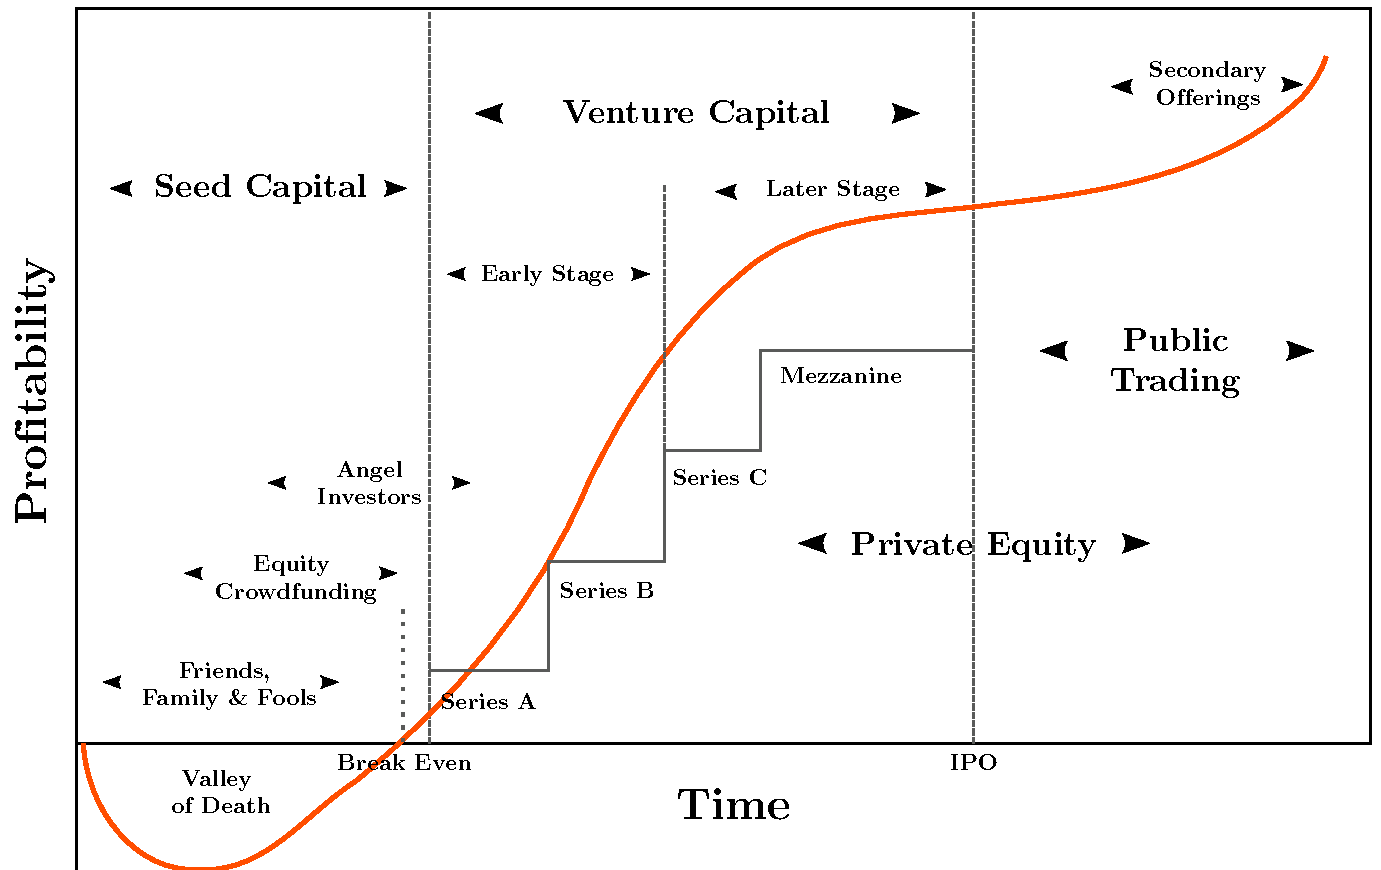
\includegraphics[width=\textwidth]{../diagrams/figures/lifecycle.pdf}
    \caption{Idealised startup development lifecycle (adapted,~\cite{lifecycle2009}). Red line represents profitability over time. Common financial instruments are labelled at times they are most likely to coincide. The chart is divided into three periods: an early period of unprofitability (``Valley of Death'') where seed capital supports the business, a period of growth sustained by rounds of venture capital, and a transition to stability and mature capital markets.}
    \label{fig:litreview:theory:lifecycle}
\end{figure}

\subsubsection{Determinants of Performance}{}

Traditional assessments of company valuation (e.g. discounted cashflows, comparable valuation) are difficult to apply to startups because they change so rapidly. Instead, when valuing startup potential we often seek more fundamental drivers. The performance of large companies is dominated by external factors: macroeconomic and industry trends, and competitor activity \cite{hansen1989}. However, startups are small and nimble enough to be largely unaffected by these factors. Rather, key determinants of startup performance are understood to be internal, flexible to changes in product and market. These determinants are often categorised into three fundamental elements: human capital, social capital and structural capital \cite{baum2004, ahlers2015}.

\begin{description}

\item[Human Capital]

Human capital is value derived from education, experience and skills \cite{gimmon2010}. Early-stage startups have little financial and structural capital and so rely on human capital to drive company growth. Human capital helps entrepreneurs identify and exploit business opportunities, define and realise their strategies, and acquire additional resources (including funding) \cite{ahlers2015}. A meta-review of human capital in startups shows industry-related experience, education and founding team compatibility contribute to startup survival \cite{gimmon2010}. Venture capitalists indicate experience and management skills are key selection criteria for early-stage startup investments \cite{gimmon2010}.

\item[Social Capital]

Social capital is value derived from relationships \cite{gedajlovic2013}. Startups require resources such as advice, finance, skills and labour to be able to realise entrepreneurial opportunities \cite{baum2004}. Social networks provide the media for those resources to be obtained. Social capital is a determinant of entrepreneurial performance, including survival time \cite{song2012}, venture capital raised \cite{gloor2013} and revenue generated \cite{stam2008}. Entrepreneurs centrally embedded in social networks are more likely to access necessary resources \cite{song2012}. Being an influencer or aligning oneself with influencers can increase the quality of an entrepreneur's connections \cite{gloor2013}. Strengthening and maintaining social networks plays an essential role in startup performance.

\item[Structural Capital]

Structural capital is value derived from intangible assets, infrastructure, and systems. Intellectual property and their proxy, patents, are a key component of structural capital, especially for early-stage startups. Innovation is a key determinant of firm survival. Patents support the appropriation of returns from innovative activities and facilitate cooperation and bargaining with business partners. Indeed, patent ownership is correlated with startup valuation \cite{hsu2008}, and leads to greater performance in terms of asset growth \cite{helmers2011} and likelihood of survival \cite{wagner2010}. Similarly, studies demonstrate a positive relationship between patent filings and startup investment \cite{hoenen2014}.

\end{description}

\subsection{Startup Investment}

Startups often seek investment from angel investors, venture capital and private equity firms. Given the uncertainty that surrounds these investment opportunities, the investment decision-making process is difficult for startups and investors alike. In this section, we discuss what motivates startups to seek investment, how investors discover and make investment decisions, and the factors that drive investment confidence.

\subsubsection{Benefits of Investment}

Many obstacles confront young companies. Startups operate using immature routines, with little knowledge of their environment and poor working relationships with customers and suppliers. In addition, startups require substantial resources to fund speculative development projects, especially when commercialising new technologies \cite{gans2003}. For these reasons, venture capital is highly desirable for entrepreneurs. Venture capital-backed firms grow faster, patent more, have higher productivity and are more likely to go public \cite{baum2004,hochberg2007}. This effect can be explained in three ways: first, investors are effective scouts of successful startups; second, investors directly help startups become successful; and third, investors send a signal that encourages other third parties (e.g. future employees, customers, investors) to support the startup.

\subsubsection{Investment Techniques}

Venture capital firms manage and invest third-party funds. Venture capital firms seek investments capable of providing financial returns and a successful exit (IPO or acquisition) within the required time frame of their fund (3–7 years). Accordingly, venture capital firms are highly selective and spend much of their time searching for potentially attractive startups and evaluating their potential for investment. There are two common approaches investors use to evaluate startup potential. First, investors extrapolate current performance metrics (e.g. app downloads, viral momentum, lifetime value of customers). Second, investors evaluate determinants of startup performance (e.g. human capital, socical capital). Regardless of approach, a key challenge for investors is informational asymmetry. Founders possess more information than investors about a startup's potential and expecting founders to transfer that knowledge to potential investors is unrealistic. To evaluate the quality of a startup's signals, investors look to factors such as third party validation (e.g. previous investments), historical performance (e.g. profitability), and contextual cues (e.g. competitor performance) \cite{ahlers2015,hoenen2014,hsu2008}.

\subsection{Proposed Framework}

External investment is a key driver of startup development. However, our understanding of factors that influence startup investment is incomplete. We discuss two key factors in investment decisions: first, evaluating startup potential and second, gauging confidence in that evaluation. Ahlers et al. \cite{ahlers2015} develop a conceptual framework for funding success on equity crowdfunding platforms. Their framework has two factors: venture quality and level of uncertainty. The first factor is based on work by Baum and Silverman \cite{baum2004} that suggests key determinants of startup potential are human capital, alliance (social) capital, and intellectual (structural) capital. The second factor is based on investors' confidence in their estimation of startup potential. We seek to generalise Ahlers' framework~\cite{ahlers2015} beyond equity crowdfunding. While the first factor of Ahlers' framework (venture quality) applies to startups of all stages, Ahlers operationalise their second factor with respect to whether startups offer an equity share in their crowdfunding, and whether they provide financial projections. These features are specific to equity crowdfunding. We propose an extension of Ahlers' framework that generalises and develops this second factor. We describe investment confidence as a product of third party validation, historical performance and contextual cues. Our proposed framework is depicted in Figure~\ref{fig:litreview:theory:framework}.

\begin{figure}[!htb]
    \centering
    
\begin{forest}
    forked edges,
    for tree={
        grow=west,
        align=center,
        l sep = 2cm,
        fork sep = 1cm,
        child anchor=east,
        anchor=base east,
        tier/.pgfmath=level(),
        edge={<-, thick},
        every node={rectangle,draw=black}
    }
[Startup\\Investment,
    [Startup\\Potential,
        [Human Capital]
        [Social Capital]
        [Structural Capital]
    ]
    [Investment\\Confidence,
        [Third Party Validation]
        [Historical Performance]
        [Contextual Cues]
    ]
]
\end{forest}

    \caption{Proposed conceptual framework for startup investment. We adapt the framework proposed by Ahlers et al.~\cite{ahlers2015}, originally based on work by Baum and Silverman~\cite{baum2004}. For an extended version of this framework, please refer to Figure~\ref{fig:appendix:features:framework}.}
    \label{fig:litreview:theory:framework}
\end{figure}

\section{Feature Selection}
\label{sec:litreview:features}

We develop a conceptual framework relating startup potential and investor confidence to startup investment. We seek to operationalise this conceptual framework into features we can incorporate into our machine learning model. Table~\ref{fig:litreview:features:summary} shows a review of features tested in previous studies of startup investment. In Appendix~\ref{chap:appendix:feature_summary}, we describe each of these features and outline conceptual and empirical evidence that justify their inclusion in our conceptual framework.

\begin{table}[!htb]
    \centering
    \scalebox{1}{
        
\newcommand{\factor}[1]{\hspace{-4em}#1}
\newcommand{\group}[1]{\hspace{-2em}#1}

\begin{tabular}{>{\hspace{4em}}lll}
\toprule
\multicolumn{1}{l}{Features} & \multicolumn{2}{c}{Results from Studies} \\
\cmidrule(lr){2-3}
 & Significant & Non-Significant \\
\midrule
\factor{Startup Potential} \\
      \group{Human Capital} \\
            Founder Capabilities
                  & \cite{beckwith2016,an2015,gimmon2010}
                  & \cite{shan2014,conti2013} \\
            Advisor Capabilities
                  & \cite{baum2004}
                  & \cite{ahlers2015,an2015} \\
            Executive Capabilities
                  & \cite{beckwith2016,an2015,conti2013}
                  & \cite{ahlers2015} \\
      \group{Social Capital} \\
            Strategic Alliances
                  & \cite{baum2004}
                  & - \\
            Social Influence
                  & \cite{beckwith2016,an2015,cheng2016,yu2015}
                  & - \\
      \group{Structural Capital} \\
            Patent Filings
                  & \cite{hoenen2014,hsu2008,baum2004}
                  & \cite{ahlers2015,gimmon2010} \\
\factor{Investment Confidence} \\
      \group{Third Party Validation} \\
            Investment Record
                  & \cite{ahlers2015,beckwith2016,croce2016,hoenen2014,conti2013}
                  & - \\
            Investor Reputation
                  & \cite{an2015,werth2013,hsu2008}
                  & \cite{hoenen2014} \\
            Media Coverage
                  & \cite{beckwith2016}
                  & \cite{an2015} \\
      \group{Historical Performance} \\
            Financial Performance
                  & \cite{beckwith2016,baum2004}
                  & - \\
            Non-Financial Performance
                  & \cite{an2015,gimmon2010}
                  & \cite{hoenen2014} \\
      \group{Contextual Cues} \\
            Industry Performance
                  & \cite{shan2014,croce2016,gimmon2010}
                  & \cite{beckwith2016,conti2013} \\
            Broader Economy
                  & \cite{beckwith2016,croce2016,hoenen2014,conti2013,hsu2008}
                  & \cite{shan2014,ahlers2015} \\
            Local Economy
                  & \cite{shan2014,beckwith2016,croce2016,gimmon2010,hoenen2014}
                  & - \\
\bottomrule
\end{tabular}

    }
    \caption{Features relevant to startup investment. We review thirteen empirical studies that investigate drivers of startup investment. For each study, we note whether included features have a significant effect on the startup investment model. We classify identified features according to our proposed conceptual framework.}
    \label{fig:litreview:features:summary}
\end{table}

Feature selection is critical to the success of our proposed conceptual framework. We build on the framework proposed by Ahlers et al. \cite{ahlers2015} in several ways. First, our framework generalises the ``Investment Confidence'' factor for startups seeking any type of investment (not just equity crowdfunding). Second, our framework has greater depth. Where Ahlers uses one or two features for each factor in their model (e.g. ``\% Nonexecutive board'' represents ``Social (alliance) capital''), we perform a review of many features employed in this area and perform a higher degree of classification. For example, in our proposed framework ``Social (alliance) capital'' is composed of ``Social influence'' and ``Strategic alliances'', each of which will also be composed of several features (e.g. ``Twitter followers'', ``Average Tweets per day'').

\section{Data Sources}
\label{sec:litreview:sources}

Predicting startup investment is a complex task. There are many features that can influence startup investment decisions. Capturing the diversity of these features is critical to developing accurate models. Accordingly, this task will likely involve data collection from multiple data sources. Appropriate selection of these data sources is important because different data sources provide insights into different actors, relationships and attributes. In Table~\ref{fig:litreview:sources:summary}, we outline the characteristics of relevant data sources and how they could contribute to our chosen features. In this section, we describe desirable characteristics of data sources for this task, review potentially relevant data sources, and ultimately determine which data sources are most likely to suit the characteristics of this task.

\afterpage{
    \clearpage
        \begin{sidewaystable}[!htbp]
            \centering
            \scalebox{0.8}{
                
\newcommand{\type}[1]{\hspace{-6em}#1}
\newcommand{\factor}[1]{\hspace{-4em}#1}
\newcommand{\group}[1]{\hspace{-2em}#1}

\begin{tabular}{>{\hspace{6em}}lcccccc}
\toprule
\multicolumn{1}{l}{Properties} & \multicolumn{2}{c}{Startup Databases} & \multicolumn{2}{c}{Social Media} & \multicolumn{2}{c}{Other Sources}\\
\cmidrule(lr){2-3} \cmidrule(lr){4-5} \cmidrule(lr){6-7}
 & CrunchBase & AngelList & LinkedIn & Twitter & PatentsView & PrivCo \\
\midrule
\type{Features} \\
      \factor{Startup Potential} \\
            \group{Human Capital} \\
                  Founders' Capabilities %DONE
                        & \cmark & \cmark
                        & \cmark\cmark & \xmark
                        & \xmark & \xmark \\
                  NED Capabilities %DONE
                        & \cmark & \cmark
                        & \cmark\cmark & \xmark
                        & \xmark & \xmark \\
                  Staff Capabilities %DONE
                        & \cmark & \cmark
                        & \cmark\cmark & \xmark
                        & \xmark & \xmark \\
            \group{Social Capital} \\
                  Social Influence %DONE
                        & \cmark & \cmark\cmark
                        & \cmark\cmark & \cmark\cmark
                        & \xmark & \xmark \\
                  Strategic Alliances %DONE
                        & \cmark & \cmark
                        & \xmark & \xmark
                        & \cmark & \xmark \\
            \group{Structural Capital} \\
                  Patent Filings %DONE
                        & \xmark & \xmark
                        & \xmark & \xmark
                        & \cmark\cmark & \xmark \\
      \factor{Investment Confidence} \\
            \group{Third Party Validation} \\
                  Investment Record
                        & \cmark\cmark & \cmark\cmark
                        & \xmark & \xmark
                        & \xmark & \cmark \\
                  Investor Reputation
                        & \cmark & \cmark\cmark
                        & \cmark & \xmark
                        & \xmark & \xmark \\
                  Media Coverage
                        & \cmark\cmark & \cmark
                        & \xmark & \cmark
                        & \xmark & \xmark \\
                  Awards and Grants
                        & \cmark & \xmark
                        & \xmark & \xmark
                        & \xmark & \xmark \\
            \group{Historical Performance} \\
                  Financial Performance
                        & \xmark & \xmark
                        & \xmark & \xmark
                        & \xmark & \cmark\cmark \\
                  Non-Financial Performance
                        & \cmark\cmark & \cmark\cmark
                        & \cmark & \xmark
                        & \xmark & \cmark \\
            \group{Contextual Cues} \\
                  Competitor Performance
                        & \cmark & \cmark
                        & \xmark & \xmark
                        & \xmark & \xmark \\
                  Broader Economy
                        & \cmark & \cmark
                        & \xmark & \xmark
                        & \xmark & \xmark \\
                  Local Economy
                        & \cmark & \cmark
                        & \xmark & \xmark
                        & \xmark & \xmark \\
\type{Ease of Use} \\
      \factor{Cost Effective}
            & \cmark & \cmark\cmark
            & \cmark & \xmark
            & \cmark\cmark & \xmark \\
      \factor{Time Efficient}
            & \cmark\cmark & \cmark\cmark
            & \xmark & \cmark\cmark
            & \cmark\cmark & \xmark \\
      \factor{Accurate Data}
            & \cmark & \cmark
            & \cmark\cmark & \cmark\cmark
            & \cmark\cmark & \cmark\cmark \\
      \factor{Large Data Set}
            & \cmark\cmark & \cmark\cmark
            & \cmark\cmark & \cmark\cmark
            & \cmark\cmark & \cmark \\
\bottomrule
\end{tabular}

            }
            \caption{Data sources relevant to startup investment. We review six data sources commonly used in entrepreneurship research for their suitability for our startup investment task. We evaluate data sources for their ability to provide relevant features for our analyses and for their ease of use in data collection. We exclude offline sources from our analyses. Ratings are: \protect\xmark~=~poor, \protect\cmark~=~satisfactory, \protect\cmark\protect\cmark~=~good.}
            \label{fig:litreview:sources:summary}
        \end{sidewaystable}
    \clearpage
}

\subsection{Source Characteristics}

Entrepreneurship studies have historically relied on surveys and interviews for data collection. Measures of human capital (e.g. founders' capabilities), strategic alliances, and financial performance are difficult to capture elsewhere. However, the trade-off for access to these features is that surveys and interviews are time-consuming and costly to implement. While online surveys address some of these issues, it is still difficult to motivate potential participants to contribute. Online data sources like startup databases and social networks are efficient because collecting data is a secondary function of users interacting with these sources. Researchers can also collect data from these sources automatically and at scale. For these reasons, we will only consider online data sources for inclusion in this study. In addition, we will restrict our scope to technology companies based in the United States. This sample is well-represented in the data sources we review. Next, we review the characteristics of online data sources commonly used in entrepreneurship research.

\subsubsection{Startup Databases}

Startup databases collect and store information about startups, investors, media coverage and trends. Most startup databases are closed systems that require commercial licenses (e.g. CB Insights, ThomsonOne, Mattermark). CrunchBase and AngelList are two crowd-sourced and free-to-use alternatives. CrunchBase and AngelList provide free Application Program Interfaces (API) for academic use. Crawlers can be developed to traverse these APIs and collect data systematically. The advantages of crawlers are that they can selectively collect data from nodes with specific attributes, collect random samples, or traverse the data source indefinitely, updating entries as new data becomes available. CrunchBase also provides pre-formatted database snapshots which allows easier access to the data set.

\begin{description}

\item[CrunchBase]

CrunchBase is an open online database of information about startups, investors, media coverage and trends, focusing on high-tech industry in the United States. It relies on its active online community to contribute to and edit most of its pages. However, this results in unpopular startups having relatively sparse profiles. CrunchBase has three provisions to prevent and remediate inaccurate crowd-sourced entries. First, users authenticate their accounts with a social media account which allows CrunchBase to verify a user's identity. Second, every change goes through a machine review, which flags significant or questionable updates. Third, established startups have their editing privileges locked and updates require manual verification.

\item[AngelList]

AngelList combines the functionality of an equity crowdfunding platform, a social networking site and an online startup database. As an equity crowdfunding platform, users create profiles for their startups on AngelList, and use the platform to attract investment. Investors use the platform to identify investment opportunities and can invest directly through AngelList, often alongside other investors in investment syndicates. AngelList is also an online startup database. It has a data-sharing agreement with CrunchBase which results in significant overlap between the two sources, though CrunchBase tends to have more comprehensive records of funding rounds \cite{cheng2016}. AngelList tracks ``startup roles'' (e.g. founders, investors, employees) with a creation-time, start-time and end-time. This means that, unlike CrunchBase, AngelList's networks can be re-created through time, which is useful for longitudinal studies.

\end{description}

\subsubsection{Social Media}

Social media platforms allow people to network and communicate online. They also capture information about peoples' identities and relationships that can be used in research. Social networking sites are diverse. Two social networks studied in detail in entrepreneurship research are LinkedIn and Twitter.

\begin{description}

\item[LinkedIn]

LinkedIn is a social network used for professional networking. It is commonly used in social network studies of entrepreneurship because it holds human capital information including past employment and education \cite{song2012}. These measures are difficult to collect elsewhere. In addition, LinkedIn can provide a measure of the professional influence of founders and investors. Unfortunately, as of May 2015, the LinkedIn API no longer allows access to authenticated users' connection data or company data \cite{trachtenberg2015}, making it difficult to use for social network analyses.

\item[Twitter]

Twitter is a social networking and micro-blogging site often used by entrepreneurs to promote their personal and business brands and share news and opportunities \cite{song2012}. Users can send and read public messages (called tweets) of 140-character length. Twitter is a directed network where users can follow other users without gaining their permission to do so. Twitter's public API provides access to social network topological features (e.g. who follows who) and basic profile information (e.g. user-provided descriptions). However, Twitter's API only provides Tweets published within the last 7 days and access to historical Twitter data requires a commercial license \cite{puschmann2013}.

\end{description}

\subsubsection{Other Sources}

\begin{description}

\item[Patent Filings]

Startups file patents to apply for a legal right to exclude others from using their inventions. In 2015, the US Patents Office (USPTO) launched PatentsView, a free public API to allow programmatic access to their database. PatentsView holds over 12 million patent filings from 1976 onwards \cite{schultz2016}. The database provides comprehensive information on patents, their inventors, their organisations, and locations. It may be difficult to match identities across PatentsView to other data sources because registered company names (as in PatentsView) are not always the same as trading names (as elsewhere).

\item[Financial Reports]

Acquiring private company financial information is difficult. Unlike public companies, private companies are not required to file with the United States Securities and Exchange Commission (or international equivalent). Proprietary databases provide some data on private companies but commercial licenses are prohibitively expensive and have poor coverage of early-stage companies. For example, PrivCo is a source for private company business and financial intelligence that covers over 500,000 private companies. PrivCo focuses its coverage on US private companies with at least \$50-100 million in annual revenues but also has some coverage on smaller but high-value private companies (like startups) \cite{artemchik2015}.

\end{description}

\subsection{Source Evaluation}

We evaluate relevant data sources for their suitability to predicting startup investment. Startup databases CrunchBase and AngelList provide the most comprehensive set of features. There are small differences between the features recorded by each. CrunchBase has slightly more coverage and tracks media better but lacks AngelList's social network and timestamping. At least one startup database should be used and either are satisfactory. Of the other data sources we review, patent filings and Twitter are most promising. PatentsView provides comprehensive patent information, though it could prove difficult matching identities to other sources. Twitter provides social network topology and basic profile information through its free API but does not provide access to historical tweets. Other data sources are less promising because of access issues. LinkedIn cannot be easily collected now the API is deprecated. Financial reports are too expensive for the purposes of this study.

\section{Learning Algorithms}
\label{sec:litreview:algorithms}

Machine learning is characterised by algorithms that improve their ability to reason about a given phenomenon given greater observation and/or interaction with said phenomenon. Mitchell provides a formal definition of machine learning in operational terms: ``A computer program is said to learn from experience E with respect to some class of tasks T and performance measure P if its performance at tasks in T, as measured by P, improves with experience E.'' \cite{mitchell1997}.

Machine learning algorithms can be classified based on the nature of the feedback available to them: supervised learning, where the algorithm is given example inputs and desired outputs; unsupervised learning, where no labels are provided and the algorithm must find structure in its input; and reinforcement learning, where the algorithm interacts with a dynamic environment to perform a certain goal. These algorithms can be further categorised by desired output: classification, supervised learning that divides inputs into two or more classes; regression, supervised learning that maps inputs to a continuous output space; and clustering, unsupervised learning that divides inputs into two or more classes.

We evaluate common machine learning algorithms with respect to their suitability for predicting startup investment. In Table~\ref{fig:litreview:algorithms:evaluation}, we rank these algorithms by cross-referencing their assumptions and properties with the task characteristics. In the following sections, we describe the characteristics of the startup investment prediction task, review common machine learning algorithms, and determine which algorithms are most likely to suit the characteristics of this task.

\afterpage{
    \clearpage
        \begin{sidewaystable}[!htbp]
            \centering
            \setlength{\extrarowheight}{.5em}
            
\newcommand{\type}[1]{\hspace{-6em}#1}
\newcommand{\factor}[1]{\hspace{-4em}#1}
\newcommand{\group}[1]{\hspace{-2em}#1}

\begin{tabular}{>{\hspace{6em}}lcccccccccccccc}
\toprule
\multicolumn{1}{l}{Criteria} & \multicolumn{14}{c}{Machine Learning Algorithms} \\
\cmidrule(lr){2-15}
 & \multicolumn{2}{l}{NB} & \multicolumn{2}{l}{LR} & \multicolumn{2}{l}{KNN} & \multicolumn{2}{l}{DT} & \multicolumn{2}{l}{RF} & \multicolumn{2}{l}{SVM} & \multicolumn{2}{l}{ANN} \\
\midrule
\type{Data Set Properties}
            & \multicolumn{2}{c}{\textbf{2}}
            & \multicolumn{2}{c}{4}
            & \multicolumn{2}{c}{6}
            & \multicolumn{2}{c}{\textbf{2}}
            & \multicolumn{2}{c}{\textbf{1}}
            & \multicolumn{2}{c}{4}
            & \multicolumn{2}{c}{6}
      \\
\midrule
      \factor{Missing Values}
            & \cmark\cmark & \cite{kotsiantis2007}
            & \cmark & -
            & \xmark & \cite{kotsiantis2007}
            & \cmark\cmark & \cite{kotsiantis2007}
            & \cmark\cmark & \cite{strobl2009}
            & \cmark & \cite{kotsiantis2007}
            & \xmark & \cite{kotsiantis2007}
      \\
      \factor{Irrelevant Features}
            & \xmark & \cite{kotsiantis2007}
            & \xmark & \cite{kuhn2013}
            & \cmark & \cite{kotsiantis2007}
            & \cmark\cmark & \cite{kotsiantis2007}
            & \cmark\cmark & \cite{strobl2009}
            & \xmark & \cite{kotsiantis2007}
            & \xmark & \cite{kotsiantis2007}
      \\
      \factor{Imbalanced Classes}
            & \cmark\cmark & -
            & \cmark\cmark & -
            & \xmark & -
            & \xmark & \cite{kotsiantis2007}
            & \cmark & \cite{strobl2009}
            & \cmark\cmark & \cite{kotsiantis2007}
            & \cmark & \cite{kotsiantis2007}
      \\
\midrule
\type{Algorithm Properties}
            & \multicolumn{2}{c}{\textbf{2}}
            & \multicolumn{2}{c}{\textbf{1}}
            & \multicolumn{2}{c}{4}
            & \multicolumn{2}{c}{4}
            & \multicolumn{2}{c}{\textbf{2}}
            & \multicolumn{2}{c}{6}
            & \multicolumn{2}{c}{6}
      \\
\midrule
      \factor{Predictive Power}
            & \xmark & \cite{caruana2008}
            & \cmark & \cite{caruana2008}
            & \cmark & \cite{caruana2008}
            & \xmark & \cite{kotsiantis2007}
            & \cmark\cmark & \cite{caruana2008}
            & \cmark\cmark & \cite{caruana2008}
            & \xmark\cmark & \cite{caruana2008}
      \\
      \factor{Interpretability}
            & \cmark\cmark & \cite{kotsiantis2007}
            & \cmark\cmark & \cite{kuhn2013}
            & \xmark & \cite{kotsiantis2007}
            & \cmark\cmark & \cite{kotsiantis2007}
            & \cmark & \cite{kuhn2013}
            & \xmark & \cite{kotsiantis2007}
            & \xmark & \cite{kotsiantis2007}
      \\
      \factor{Processing Speed} %TODO
            & \cmark\cmark & \cite{kotsiantis2007}
            & \cmark\cmark & \cite{caruana2008}
            & \cmark\cmark & \cite{kotsiantis2007}
            & \cmark & \cite{kotsiantis2007}
            & \cmark & \cite{caruana2008}
            & \xmark  & \cite{kotsiantis2007}
            & \xmark  & \cite{kotsiantis2007}
      \\
\midrule
\type{Overall}
            & \multicolumn{2}{c}{\textbf{2}}
            & \multicolumn{2}{c}{\textbf{2}}
            & \multicolumn{2}{c}{6}
            & \multicolumn{2}{c}{4}
            & \multicolumn{2}{c}{\textbf{1}}
            & \multicolumn{2}{c}{5}
            & \multicolumn{2}{c}{7}
      \\
\bottomrule
\end{tabular}

            \caption{Evaluation of machine learning algorithms for startup investment prediction. We review seven common supervised machine learning algorithms for their suitability for our startup investment task. We evaluate algorithms for their robustness to the structure of the data set and their appropriateness for the constraints of our implementation. We rank the algorithms according to the sum of these measures (in each section and overall) and bold highly-ranked algorithms. Ratings are: \protect\xmark~=~poor, \protect\cmark~=~satisfactory, \protect\cmark\protect\cmark~=~good. Algorithms are: NB~=~Naive Bayes, LR~=~Logistic Regression, KNN~=~K-Nearest Neighbours, DT~=~Decision Trees, RF~=~Random Forests, SVM~=~Support Vector Machines, ANN~=~Artificial Neural Networks.}
            \label{fig:litreview:algorithms:evaluation}
        \end{sidewaystable}
    \clearpage
}

\subsection{Task Characteristics}

Machine learning tasks are diverse. Our investigation into startup investment is a task that suits supervised machine learning algorithms. We will manipulate the data we collect into a single labelled data set. Startups will be labelled based on whether they receive investment at each funding round (Seed, Series A, B etc.). We may also investigate measures of startup performance (e.g. survival time, exit). The key objective of machine learning algorithm selection is to find algorithms that make assumptions consistent with the structure of the problem (e.g. tolerance to missing values, mixed feature types, imbalanced classes) and suit the constraints of the desired solution (e.g. time available, incremental learning, interpretability). In the following sections, we outline the characteristics of supervised learning tasks relevant to our startup investment prediction task.

\subsubsection{Data Set Properties}

\begin{description}

\item[Missing Values]

Data sets often have missing values, where no data is stored for a feature of an observation. Missing data can occur because of non-response or due to errors in data collection or processing. Missing data has different effects depending on its distribution through the data set. Public data sets, like startup databases and social networks, are typically sparse with missing entries despite their scale. Therefore, robustness to missing values is a desirable property of our algorithm.

\item[Mixed Feature Types]

Data sets can contain data with distinct primitive natures: real-valued, interval, counts, rank, binary, ordinal, categorical and multi-categorical types. The simplest way to handle mixed feature types is to convert into a unified type (e.g. real-valued, binary). However, this process partially discards type-specific information. We expect mixed feature types in our data set as we will be handling data from databases, social networks and semantic text analysis. Therefore, robustness to mixed feature types is a desirable property of our algorithm.

\item[Irrelevant Features]

Despite efforts to only include features that have theoretical relevance, machine learning tasks often include irrelevant features. Irrelevant features have no underlying relationship with classification. Depending on how they are handled they may affect classification or slow the algorithm. We expect irrelevant features in our data set because our proposed framework includes features that have not been thoroughly tested in the literature. Therefore, robustness to irrelevant features is a desirable property of our algorithm.

\item[Imbalanced Classes]

Data sets are not usually restricted to containing equal proportions of different classes. Significantly imbalanced classes are problematic for some classifiers. In the worst case, a learning algorithm could simply classify every example as the majority class. Our data set is not dramatically imbalanced overall, but when looking at funding status for different funding rounds it is significantly imbalanced. Therefore, robustness to imbalanced classes is a desirable property of our algorithm.

\end{description}

\subsubsection{Algorithm Properties}

\begin{description}

\item[Predictive Power]

Predictive power is the ability of a machine learning algorithm to correctly classify new observations. Predictive power can be evaluated in many ways. As our data set is likely to have an imbalanced class distribution, we will evaluate predictive power based on balanced metrics like Area under the Receiver-Operator Curve and the F1 Score. If a model has no predictive power, then the model is not representing the underlying process being studied. For this reason, predictive power is a desirable property of our algorithm. However, if multiple algorithms provide similar predictive power other selection criteria become significant too.

\item[Interpretability]

Interpretability is the extent to which the reasoning of a model can be communicated to the end-user. There is a trade-off between model complexity and model interpretability. Some models are a ``black box'' in the sense that data comes in and out but the model cannot be interpreted. For this study, it is a key objective that we improve our understanding of the determinants of startup investment. Therefore, interpretability is a desirable property of our algorithm.

\item[Incremental Learning]

Incremental learning is where learning occurs dynamically whenever new observations are made and the algorithm adjusts what has been learned per the new observations. The key driver behind the need for incremental learning is when the underlying source generating the data is changing. It is plausible that, as a system, the drivers behind startup investment change over time. Incremental learning will allow us to gain an understanding of whether that is accurate. Therefore, incremental learning is a desirable property of our algorithm.

\end{description}

\subsection{Algorithm Characteristics}

Supervised machine learning are algorithms that reason about observations to produce general hypotheses that can be used to make predictions about future observations. Supervised machine learning algorithms are diverse, from symbolic (Decision Trees, Random Forests) to statistical (Logistic Regression, Naive Bayes, Support Vector Machines), instance-based (K-Nearest Neighbours), and perceptron-based (Artificial Neural Networks). In the following sections, we describe each candidate learning algorithm, critique their advantages and disadvantages, and present evidence of their effectiveness in applications relevant to startup investment.

\subsubsection{Naive Bayes}

Naive Bayes is a simple generative learning algorithm. It is a Bayesian Network that models features by generating a directed acyclic graph, with the strong (naive) assumption that all features are independent. While this assumption is generally not true, it simplifies estimation which makes Naive Bayes more computationally efficient than other learning algorithms. Naive Bayes can be a good choice for data sets with high dimensionality and sparsity as it estimates features independently. Naive Bayes sometimes outperforms more complex machine learning algorithms because it is reasonably robust to violations of feature independence \cite{kotsiantis2007}. However, Naive Bayes is known to be a poor estimator of class probabilities, especially with highly correlated features \cite{niculescu2005}. Naive Bayes was used alongside Logistic Regression, Decision Trees and Support Vector Machines to predict success in equity crowdfunding campaigns on the AngelList data set \cite{beckwith2016}. None of these models performed well. The algorithm that best predicts startup investment was Naive Bayes with a Precision of .41 and Recall of .19, which means only 19\% of funded startups were classified correctly by the model. The author suggests the poor performance of their algorithms is caused by features not captured in their data set relating to Intellectual Capital, Third Party Validation and Historical Performance. These features will be included in this study.

\subsubsection{Logistic Regression}

Regression is a class of statistical methods that investigates the relationship between a dependent variable and a set of independent variables. Logistic regression is regression where the dependent variable is discrete. Like linear regression, logistic regression optimises an equation that multiplies each input by a coefficient, sums them up, and adds a constant. However, before this optimisation takes place the dependent variable is transformed by the log of the odds ratio for each observation, creating a real continuous dependent variable on a logistic distribution. A strength of Logistic Regression is that it is trivial to adjust classification thresholds depending on the problem (e.g. in spam detection \cite{friedman2001}, where specificity is desirable). It is also simple to update a Logistic Regression model using online gradient descent, when additional training data needs to be quickly incorporated into the model (incremental learning). Logistic Regression tends to underperform against complex algorithms like Random Forest, Support Vector Machines and Artificial Neural Networks in higher dimensions \cite{caruana2008}. This underperformance is observed when Logistic Regression is applied to startup investment prediction tasks \cite{beckwith2016, bhat2011}. However, weaker predictive performance has not prevented Logistic Regression from being commonly used. Its simplicity and ease-of-use means it is often used without justification or evaluation \cite{gimmon2010}.

\subsubsection{K-Nearest Neighbours}

K-Nearest Neighbours is a common lazy learning algorithm. Lazy learning algorithms do not produce explicit general models, but compare new instances with instances from training stored in memory. K-Nearest Neighbours is based on the principle that the instances within a data set will exist near other instances that have similar characteristics. K-Nearest Neighbours models depend on how the user defines distance between samples; Euclidean distance is a commonly used metric. K-Nearest Neighbour models are stable compared to other learning algorithms and suited to online learning because they can add a new instance or remove an old instance without re-calculating \cite{kotsiantis2007}. A shortcoming of K-Nearest Neighbour models is that they can be sensitive to the local structure of the data and they also have large in-memory storage requirements. K-Nearest Neighbours was compared to Artificial Neural Networks to predict firm bankruptcy \cite{ahn2008}. K-Nearest Neighbours is attractive in bankruptcy prediction because it can be updated in real-time. By optimising feature weighting and instance selection, the authors improved the K-Nearest Neighbours algorithm to the extent that it outperformed the Artificial Neural Networks.

\subsubsection{Decision Trees}

Decision Trees use recursive partitioning algorithms to classify instances. Each node in a Decision Tree represents a feature in an instance to be classified, and each branch represents a value that the node can assume. Methods for finding the features that best divide the training data include Information Gain and Gini Index \cite{kotsiantis2007}. Decision Trees are close to an ``off-the-shelf'' learning algorithm. They require little pre-processing and tuning, are interpretable to laypeople, are quick, handle feature interactions and are non-parametric. However, Decision Trees are prone to overfitting and have poor predictive power \cite{caruana2006}. These shortcomings are addressed with pruning mechanisms and ensemble methods like Random Forests, respectively. Decision Trees were compared with Naive Bayes and Support Vector Machines to predict investor-startup funding pairs using CrunchBase social network data \cite{liang2016}. Decision Trees had the highest accuracy and are desirable because their reasoning is easily communicated to startups.

\subsubsection{Random Forests}

Random Forests are an ensemble learning technique that constructs multiple Decision Trees from bootstrapped samples of the training data, using random feature selection \cite{breiman2001}. Prediction is made by aggregating the predictions of the ensemble. The rationale is that while each Decision Tree in a Random Forest may be biased, when aggregated they produce a model robust against over-fitting.  Random Forests exhibit a performance improvement over a single Decision Tree classifier and are among the most accurate learning algorithms \cite{caruana2006}.  However, Random Forests are more complex than Decision Trees, taking longer to create predictions and producing less interpretable output. Random Forests were used to predict private company exits using quantitative data from ThomsonOne \cite{bhat2011}. Random Forests outperformed Logistic Regression, Support Vector Machines and Artificial Neural Networks. This may be because the data set was highly sparse, and Random Forests are known to perform well on sparse data sets \cite{breiman2001}.

\subsubsection{Support Vector Machines}

Support Vector Machines are a family of classifiers that seek to produce a hyperplane that gives the largest minimum distance (margin) between classes. The key to the effectiveness of Support Vector Machines are kernel functions. Kernel functions transform the training data to a high-dimensional space to improve its resemblance to a linearly separable set of data. Support Vector Machines are attractive for many reasons. They have high predictive power \cite{caruana2006}, theoretical limitations on overfitting, and with an appropriate kernel they work well even when data is not linearly separable in the base feature space. Support Vector Machines are computationally intensive and complicated to tune effectively (compared to Random Forests, for example). Support Vector Machines were compared with back propagated Artificial Neural Networks in predicting the bankruptcy of firms using data provided by Korea Credit Guarantee Fund \cite{shin2005}. Support Vector Machines outperformed Artificial Neural Networks, possibly because of the small data set.

\subsubsection{Artificial Neural Networks}

Artificial Neural Networks are a computational approach based on a network of neural units (neurons) that loosely models the way the brain solves problems. An Artificial Neural Network is broadly defined by three parameters: the interconnection pattern between the different layers of neurons, the learning process for updating the weights of the interconnections, and the activation function that converts a neuron's weighted input to its output activation. A supervised learning process typically involves gradient descent with back-propagation \cite{rumelhart1988}. Gradient descent is an optimisation algorithm that updates the weights of the interconnections between the neurons with respect to the derivative of the cost function (the weighted difference between the desired output and the current output). Back-propagation is the technique used to determine what the gradient of the cost function is for the given weights, using the chain rule. Artificial Neural networks tend to be highly accurate but are slow to train and require significantly more training data than other machine learning algorithms. Artificial Neural Networks are also a black box model so it is difficult to reason about their output in a way that can be effectively communicated. Artificial Neural Networks are rarely applied to startup investment or performance prediction because research in this area typically uses small and low-dimensional data sets. As one author puts it ``More complex classification algorithms—artificial neural networks, Restricted Bolzmann machines, for instance—could be tried on the data set, but marginal improvements would likely result.'' \cite{beckwith2016}. However, this study will address these issues so Artificial Neural Networks may be more competitive.

\subsection{Algorithm Evaluation}

We evaluate supervised learning algorithms for their suitability in startup investment prediction. While our evaluation gives us directionality of fit, we hesitate to discard algorithms based on our literature review. Algorithm selection is complex and preliminary testing will provide clarity as to which algorithms should be used. In addition, larger training sets and good feature design tend to outweigh algorithm selection \cite{caruana2008}. With those concessions in mind, our findings suggest we expect Random Forests, Support Vector Machines and Artificial Neural Networks to produce the highest classification accuracies. An ensemble of these algorithms may improve accuracy further, though at the cost of computational speed and interpretability. We may expect Random Forests to outperform the other two algorithms due to robustness to missing values and irrelevant features and native handling of discrete and categorical data. However, Random Forests are not highly interpretable so Decision Trees and Logistic Regression may be preferable for exploratory analysis of the data set.

\section{Conclusion}
\label{sec:litreview:conclusion}

%Overview

We conduct a literature review to determine the factors that influence investment for startups. First, we explore theoretical models of technology startups and startup investment (Section~\ref{sec:litreview:theory}). Thereafter, we reviewe empirical evidence of features linked to startup investment (Section~\ref{sec:litreview:features}). We determine how to collect the data to test those features (Section~\ref{sec:litreview:sources}) and evaluate machine learning algorithms to find those that suit startup investment prediction (Section~\ref{sec:litreview:algorithms}).

%Rationale

Venture capital funding for late-stage privately-held startups is approaching all-time highs as investors enter the private markets \cite{nvca2016}. It is important to understand how the factors that influence venture capital investment change throughout a startup's development. There is a substantial research gap around predicting startup investment. Existing approaches in the literature have three common limitations: small sample size \cite{ahlers2015, gimmon2010, dixon2014, hoenen2014, yu2015, an2015, werth2013, croce2016}, a focus on early-stage investment \cite{beckwith2016, ahlers2015, cheng2016, yuan2016, croce2016}, and sparse use of features \cite{ahlers2015, an2015, cheng2016, croce2016, werth2013, gimmon2010}. Although individual studies address some of these limitations, none attempt to synthesise their findings into a standalone study and software design.

%Implications

This study will develop software that collects and processes information on startups to predict their likelihood of raising investment at different stages in their development. If successful, this study has the potential for scholarly, policy and firm-specific implications. We propose a conceptual framework for startup investment, based on work by Ahlers et al. \cite{ahlers2015} and Baum and Silverman \cite{baum2004}. Our conceptual framework models startup investment as a product of two factors: startup potential and investment confidence. We will test this framework with respect to startup development, using cross-sectional and longitudinal analyses. Our aim is that this study improves our understanding of the determinants of startup investment, especially in later-stage startups. Ultimately, we hope this study encourages greater investment in startups.

\appendix

\chapter{Feature Summary}
\label{chap:appendix:feature_summary}
\subfile{appendix}

\printbibliography
\end{refsection}

\chapter{Original Honours Proposal}
\label{chap:appendix:original_proposal}
\subfile{../proposal/original_proposal}

\chapter{Revised Honours Proposal}
\label{chap:appendix:revised_proposal}
\subfile{../proposal/revised_proposal}


\end{document}

